\documentclass[a4paper]{article}

%% Language and font encodings
\usepackage[english]{babel}
\usepackage[utf8x]{inputenc}
\usepackage[T1]{fontenc}
\usepackage{float}

%% Sets page size and margins
\usepackage[a4paper,top=3cm,bottom=2cm,left=3cm,right=3cm,marginparwidth=1.75cm]{geometry}

%% Useful packages
\usepackage{amsmath}
\usepackage{graphicx}
\usepackage{listings}
\usepackage[colorinlistoftodos]{todonotes}
\usepackage[colorlinks=true, allcolors=black]{hyperref}

\title{Matchpool}
\author{Philip Saunders, Yonatan Ben Shimon}

\begin{document}
\maketitle
\begin{abstract}
Matchpool is a decentralized matchmaking protocol which uses group dynamics to help as many participants as possible to find love. It can also be used as a more generic platform for any kind of paid membership community which can clearly define two sides of an interaction or market. This paper presents the elements of the platform: the Ethereum smart contracts which handle the trust-sensitive ownership and reward structures, as well as the core game logic which makes it work. Finally we lay out a two year roadmap for launching and scaling the network, including a detailed specification of the Guppy token (GUP), which will play an integral role in its development.
\end{abstract}

\tableofcontents

\section{Introduction}

Most dating apps on the market today suffer from two core flaws. Firstly, there is a tendency to rely on dehumanizing profiling strategies, to the exclusion of more effective forms of matching. Secondly, eager for subscription money, many apps often allow huge demographic imbalances to occur to the detriment of user experience. In a study by the GlobalWebIndex it was estimated that over 62\% of location-based dating apps such as Tinder are used by men. Where Tinder is concerned, the abundance of men and the scarcity of women, mixed with a lack of real life social cues creates an environment that is neither fun nor ultimately successful for most users.

Matchpool solves these game-theoretic problems by allowing users to create pools in their area with custom demographic specifications. Pools can be visualized as a cross between Slack channels and Meetup groups- federated, invite-only groups owned and run by devoted matchmakers. In this paper, we will describe the process by which matchmakers are rewarded in the network's internal token for matching new entrants successfully. The quality or reputation of particular pools is measured against whether the joiner's particular goals have been met.

What makes Matchpool unique is the matchlock feature, which keeps a 50:50 ratio between x and y. If a certain number of x users enters the pool, then the matchlock will stop more x from entering until the same number of y’s arrive. In a dating context this could apply to gender, but it can also be parameterized to any use case where any arbitrary market polarity is required. Also, there is no restriction requiring the x and y side of the matchlock to be opposites. For entrepreneurial networking or any other use case the x and y can be identical (or completely unset). For LGBT dating pools the "gender" configuration of both sides could be the same. It is up to the pool founder to configure the matchlock according to the kind of community they wish to create.

\section{Strategies}

\textit{Social networks have two strategies for connecting users: profiling and pooling.}

Before the internet, a typical profiling strategy for social networking would be something like a “classified” in the local paper. This might be effective for advertising products or vacancies where both sides are clear about what they want. A good current example of where this approach works well is the job marketplace Indeed.com. Some users advertise what they are looking for, and other users compete to meet that demand.

Then there's Twitter, at the other extreme. On Twitter, users have a profile for sure, but most activity emerges spontaneously from human interaction. This is an example of a social network geared primarily towards pooling. Pooling strategies applied to dating in the real world include things like bars, nightclubs, dancing, as well deliberate forms of matchmaking like speed-dating. All of these activities have an underlying element of ritual distraction, which people need to get over themselves. This important element has been recognized and practiced throughout human history, but is missing from more atomized online approaches.

Matchpool implements a combination of the two. Joiners do have profiles, but only for sorting into pools, after which they can participate in pool chats, play dapplets and go to events (organized by the matchmaker for the group as a whole) or dates with other pool members. The basic philosophy of pools is to creating the right environment and then letting nature take its course.

While pools have a direct interest in creating as many matches as possible, we assume singles are already motivated. Once inside a pool, there is little unnecessary mediation. By creating an intentional high trust community, there is a subtle pressure to behave better and not engage in spamming or low-quality mass messaging. There is a tendency in blockchain development and systems design to lean heavily on boilerplate notions of “reputation” and “incentives”, while ignoring the fact that reputation is a complex, emergent property of other people's subjective impressions and market decisions. Groups allow for this kind of unmeasured (and unmeasurable) “reputation” to emerge among their members without the need for some contrived score or karma count. Quantified reputation only relates to the quality of the pool as a whole, not to individual participants.

\section{Participants}
\textit{There are two kinds of participants on Matchpool: joiners and hosts. }

\subsection{Joiners}

\begin{figure}[!ht]
\centering
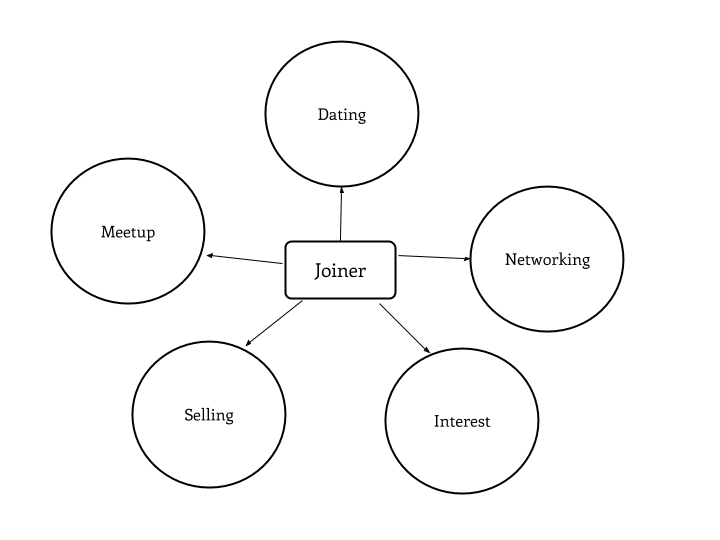
\includegraphics[width=0.5\textwidth]{pools.png}
\end{figure}

Joiners are a self-explanatory category: anyone who wants to join a pool with the intention of meeting someone that matches their particular interest. Joiners have the following rough user journey:

\begin{enumerate}
\item
User supplies a number of "factors", or details about themselves: name, age, gender, interests, personality type, sexual orientation, seeking relationship type, education level, income, ethnicity, religion, fitness, etc. This data is confidential and encrypted, and only used for the purpose of matching people into pools.
\item
User creates a wallet and has the option to buy Guppies, either to exchange it from crypto or to purchase it directly with fiat using their credit card. This is for the purpose of paying the entry fee into pools.
\item
User can see the various pools which exist within geographical proximity to their location. Depending on the values they have provided, they will see pools they are qualified for.
\item
User enters the pool of their choice and pays the requisite entry fee (if applicable to the business model of the pool and other policies which can be put in place).
\item
New entrants have a higher reward rate for matchmakers to pair them up. During this initial period, date seekers will likely be matched with several people.
\item
When users go on a date it is published in their “notebook”, which is a public log of activities. The process of logging an event involves agreement with the other person before it appears.
\item
Users can go to events, message other date seekers, play dapplets and go on dates until they are in a relationship, at which point their journey is complete. They have the option to remain a member of the pool and act as a matchmaker for other dateseekers (thereby earning divs) or leave.
\end{enumerate}

Joiners are billed by the pool monthly for membership. All billing in Matchpool is denominated in the network's native token, Guppies (GUP). Joiners can act as "helpers" to the pool host, for example as a matchmaker, admin or greeter.

\subsection{Hosts}

The host is the founder of the pool and sets in place the specifications regarding who can become a member. A helper, on the other hand, can be any member within the pool who acts as a matchmaker for other members. Helpers propose matches between two other joiners who they believe would be good partners. Depending on the kind of proposed match: a date, a relationship, or a marriage; the helper will get a different number of matchpoints. \textbf{Table 1} shows a sample breakdown of the reward system.

\begin{table}[!h]
\centering
\begin{tabular}{l|r}
Action & Value \\\hline
Date & 1 matchpoints \\
Meeting & 1 matchpoints \\
Relationship & 20 matchpoints \\
Engagement & 150 matchpoints
\end{tabular}
\caption{\label{tab:widgets}Action-to-value list, configured by host.}
\end{table}

This is not the exact number; this will be determined via trial and error. The process for all of these “matches” is in 4 steps.

\begin{enumerate}
\item
Anyone can start a pitch involving two other users with an event category: Bob, Alice - Date.
\item
Bob and Alice are notified, and can accept or reject.
\item
If they both accept, the event is added to their public notebook, which is a log of activity.
\item
The proposer earns 1 matchpoint.
\end{enumerate}

The trust model of this interaction assumes a few things. Since a) both Bob and Alice are paying for membership of the pool and b) their identities have been verified, they have no incentive to accept the match fraudulently. The event is also posted to both of their public notebooks (similar to a Facebook relationship status update). In the Matchpool app there will be all the functionality for scheduling and arranging events as well as "Stories" after the event has happened.

Use section and subsections to organize your document. Simply use the section and subsection buttons in the toolbar to create them, and we'll handle all the formatting and numbering automatically.

Matchpoints, first of all, entitle the matchmaker to a certain share of divs in the pool. Divs entitle the owner to a certain share of the monthly subscription revenue.

Once matchmakers have collected a certain number of arrows, they have the ability to start new pools.

\section{Pools}

\textit{Love is composed of a single soul inhabiting two bodies.} - Aristotle

\subsection{Overview}
A pool is the basic unit in Matchpool, which features a Slack-like public chat interface as well as the ability to send private messages along with other features including a wallet. Pools are established by matchmakers in two ways. The first way is to reserve in escrow a certain number of Matchpool tokens (“guppies”) which is held in the pool for the duration that it is open. The second method is users who have acquired a certain number of arrows from matching people in other pools can create them. Since successful matchmaking is a vital component of the public reputation of pools and the network as a whole, it is important that new pools should be started by people who have a successful track record.

\subsection{Matchlock}
The matchlock allows the host to configure the demographic details of two sides of the interaction- X and Y. When starting a pool, the host is able to configure the matchlock with the required factors for each side of the interaction, including gender, age-range, education level, ethnicity, religion and geographical proximity. This can be as broad and detailed or generic.

When a certain number of type X enters, the pool becomes unavailable to users of type X until the same number of type Y enters. One of the issues with the matchlock is that people may be compelled to change their details in order to get around the matchlock. However, we will develop a number of mechanisms in the platform which will allow for peer authentication and dispute of factors, including social media verification.

The population limit is set to 144 by default, which is approximately Dunbar’s Number- the number of personal relationships that the human mind can handle. But the host can also configure this parameter if a larger or smaller limit is desired.

Table 2 is an example of how the host can configure the matchlock, with each field having its own set of valid factors. Users who are registered on the protocol with that list of factors can then be matched to their group of choice, as long as the matchlock is not activated due to demographic imbalance.

\begin{table}[!h]
\centering
\begin{tabular}{l|r}
X & Y \\\hline
Female & Male \\
21-35 & 21-35 \\
Some College & Some College \\
0-20km & 0-10km \\
10 GUP & 20 GUP
\end{tabular}
\caption{\label{tab:widgets}A list of example demographic configurations for the matchlock }
\end{table}


\subsection{Finding Pools}
Matchpool will implement a front-end interface which will allow users to search for pools in different areas, matched with different interests. In this respect it will be somewhat similar to Meetup.com; users can search various factors to see if something fits. In the on-boarding process they will also be shown a list of pools in their area which fits their particular demographics and interests.

\subsection{Fee Options}

The matchlock configuration also defines the entry fee in the protocol's internal currency for different groups as well as the ongoing monthly subscription fee. In the example of a dating pool, this is important because there may be a great deal of variation between demand coming from males than females; in which case it would make sense for the price to be more expensive for one and cheaper (or even free) for others. The lock will prevent any demographic imbalances from occurring, however, when a user for whatever reason is unable to enter a locked pool, they can “register interest” in joining. Based on these interest indicators, the host will be able to see the demand level and adjust the price accordingly.

\subsection{Notebooks}
The notebook is a kind of log which all Matchpool users have. This log updates with events such as dates, relationship status update and “stories”. Whenever a user goes on a date they have the option to share a story of how it went, which is added to their public notebook.

\subsection{Dapplets}
Dapplets are add-ons created by developers who want add to the Matchpool protocol. In practice, Dapplets work similar to Slack plugins but can enhance the experience in a number of ways. One example would be a dapplet which implements “Tinder” functionality: users can swipe through other users.

A good example of where this works well is on sites like MeetMe.com, which had a suite of mini-games like "Lunch Money", "Blind Date" etc. which helped users meet and get to know each other.

Dapplet developers are rewarded similarly to Matchmakers: if one of their apps creates a match of some kind, the dapplet developer earns arrows which translate into divs. In the same way that an individual within a group can pitch a match between x and y, so can a game. For example, if a "Blind Date" game creates a real match, then the dapplet developer will earn the same number of arrows and be rewarded via the same process as manual social match within the pool.

We will develop a dapplet marketplace so that pools can continuously incorporate new functionality.

\section{Ownership Logic}

\subsection{Matchpoints}
Joiners pay a certain fee for continual membership of pools, which is payable monthly. This payment is made to host. The host can operate as a matchmaker themselves within the pool, but other members can also act as helpers, as mentioned earlier. Whenever a matchmaker achieves a successful pitch, defined by whether two people mutually update their Matchpool notebooks to reflect the event, they are awarded “matchpoints”. The host, as the owner and founder of the pool, automatically has a share. An automatic share can be allocated to cupids too, but for the most part this is a breakdown of what this might look like.

\begin{figure}[!ht]
\centering
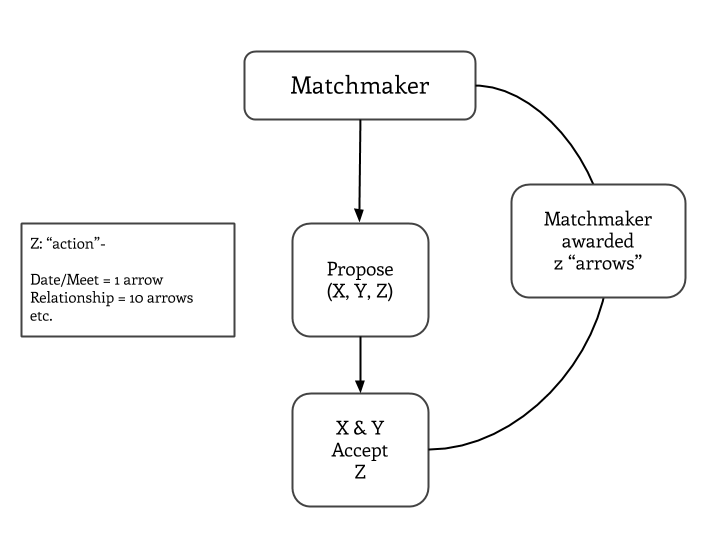
\includegraphics[width=0.5\textwidth]{arrowjourney.png}
\caption{\label{fig:Matchmakers} The process of Pitching.}
\end{figure}

\subsection{Divs}
Over every epoch a pool makes a certain amount of revenue, based on member subscriptions. Divs decide who owns this revenue. If a pool makes 2000 GUP over a given epoch, and a user holds at 50\% of the divs in that pool, they will receive 1000 GUP at the end of the epoch. Until that point, the funds are held in escrow in the smart contract and cannot be moved.

\begin{figure}[!ht]
\centering
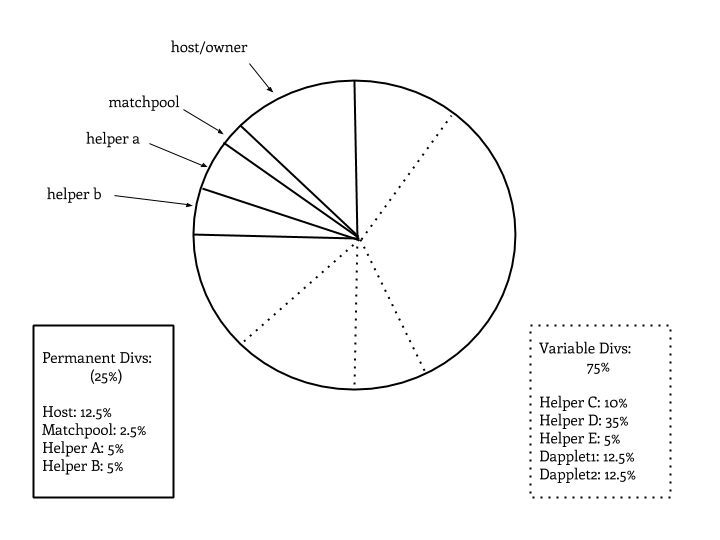
\includegraphics[width=0.5\textwidth]{divs.png}
\caption{\label{fig:Matchmakers} Perms and Vars denominated as one.}
\end{figure}

There are two categories of divs: \textbf{permanent divs} and \textbf{variable divs}. Variable divs are calculated using the following formula:

\[\frac{totalrevenue * tempdivs}{100} * \frac{earnedarrows}{totalarrows} \][!h]

This follows a few steps.
\begin{enumerate}
\item
Get the total revenue (intake of Guppies) then find the amount that is allocated to variable divs.
\item
Find the users divs by calculating the number of arrows accumulated as a percentage of the total arrows created during that epoch.
\item
Multiply them to find the amount due to the user.
\end{enumerate}
Permanent divs are pre-determined by the owner/owners of the pool, who can choose to grant divs to anyone. The share left over from permanent divs are given over to helpers who match other users on the platform, as described earlier in this paper. This is a breakdown of permanent and temporary divs considered seperately.

\begin{figure}[!ht]
\centering
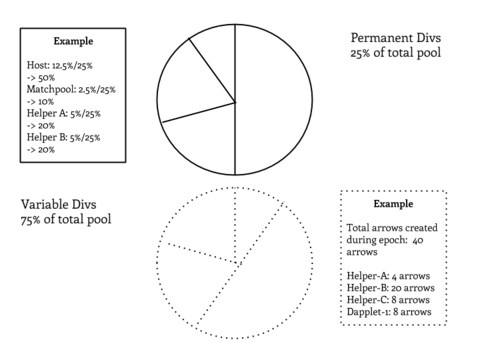
\includegraphics[width=0.5\textwidth]{permanent-temporarydivs_480.png}
\caption{\label{fig:Matchmakers} Perms and Vars considered separately.}
\end{figure}

\subsection{Other Business Models}
There are four basic business models available to hosts:
\begin{itemize}
\item
Entry fee
\item
Subscription
\item
Packages
\item
Pay on delivery
\end{itemize}
Some pools may want to have alternate business models, for example to implement an escrow contract that pays half initially and half on delivery. We will facilitate these business models by implementing them in the form of dapplets. The monthly subscription facility for membership will itself be a dapplet, while a single membership with escrow will be another option. When Matchpool launches we will provide a basic suite of dapplets that hosts can configure while opening up the API to allow developers to contribute custom models.

\section{Privacy}
The factors that define a user's demographics are private by default, and only revealed to other users on the platform with the users explicit consent. In the last few years there has been a struggle between the interests of internet users and the interests of governments on the topic of strong cryptography. Matchpool will be incorporated in a territory which will best allow for complete privacy for users. We will also design the platform in such a way as to avoid holding centralized databases. This is important to avoiding hacking of users data.

One of the potential pitfalls is that people will use the network for socially undesirable purposes, such as prostitution or selling drugs. At the end of the day Matchpool cannot control exactly how people use it. What we can do is provide the software and implement tools so that people are able to distinguish good pools from bad. One such feature is that all pools will be equipped with a public profile so that people can review and share stories about their experience within it. If pools are used for socially undesirable purposes then it will become quickly apparent. Ultimately it is up to the community, which has a stake in its success, to create and join environments which reflects their values.

\section{Trust Policy}
\subsection{Centralization vs Decentralization}
One of the major themes of the crypto community has been on the importance of the concept of decentralization. The origin of this theme was Satoshi Nakamoto's conception of Bitcoin as a "trustless" currency- which doesn't rely on a particular authority to guarantee the truth of its record. In the context of apps, decentralization is not an unlimited good in and of itself.

Therefore trust policy of Matchpool breaks down into three categories:
\begin{itemize}
\item
Decentralized.
\item
Federated.
\item
Centralized.
\end{itemize}

The trust-sensitive aspects of the cryptocurrency and arrows are decentralized and can't be meddled with. This is also true for the core protocol.

However, apps and platforms rely on continual development to stay competitive. Continual development requires developers to have permissioned access to update the software constantly. So the front-end will be centralized and under the control of Matchpool as an organization. Here is the breakdown:

\begin{table}[!h]
\centering
\begin{tabular}{c|c|c}
Centralized & Federated & Decentralized \\\hline
Front-end & Div distrdibution & Cryptocurrency \\
Pool deletion & Pool admission & Arrows \\
& User banning & Div payments \\
& Arrow rewards &

\end{tabular}
\caption{\label{tab:widgets} Matchpool's trust policy }
\end{table}

\subsection{Pool Banning}

There are some cases where it might be necessary to delete pools that violate the law. This is part of Matchpool’s use policy which users consent to when signing up. This would include behaviours that are clearly against the law of jurisdictions where Matchpool is used, such as  child pornography and human trafficking. We will use a flagging process and an application form where the complainant would have the ability to include screenshots. Since pools are encypted Matchpool would not be able to read public pool chats; it relies on a combination of public pool reviews on the outside as well as the reporting mechanism. The Matchpool organization would have the centralized ability to delete the pool in question from the app.

We distinguish between Matchpool as an app and Matchpool as a protocol. The protocol is open for anyone to use an API directly; for example for divs and points. However the app is a service we are offering the Matchpool community. If a pool is deleted the entity within the smart contract would remain for users who still have divs and Guppies in the relationship in question. We will try to find the best balance between good community governance and protection of privacy and liberty of joiners.

\subsection{Contracts}

The core Matchpool protocol which deals with the “rules” of the game is decentralized using the Ethereum Virtual Machine (EVM). Ethereum is a programmable blockchain which can run small units of code called smart contracts. Blockchains have become something of a buzzword so it's a good idea to explain what they are and what they're useful for- and more importantly, what they're not useful for.
A “blockchain” in general is a peer-to-peer network where every member (node) holds the same copy of a shared record or database, which can't be defrauded. In the case of Bitcoin, this shared record behaves as a simple ledger of addresses and balances of Bitcoin currency.

Blockchains are highly useful for trust-sensitive use cases where having a particular institution controlling it would lead to conflicts of interest where there is a risk of exploiting trust counter to users. In proof-of-work blockchains, new entries can only be added to the record by solving mathematical puzzles and providing cryptographic proof that the node has solved the puzzle. When this happens, the node is allowed to add a certain number of transactions to a “block”, which is appended to the blockchain, making the record one block higher. Ethereum adds to the core functionality of ledger-based blockchains by adding in a “Turing-Complete” scripting language called Solidity which can compile directly into EVM opcodes. Turing-completeness is another buzzword which means a language where any imaginable problem could theoretically be expressed and solved, although it should be noted that in Ethereum there is a limit to this complexity imposed by network charges, expressed in gas.

\section{Guppies}
\subsection{The Purpose of Having a Token}
Why not simply denominate all interactions on the platform in terms of Ether or another well known cryptocurrency instead of creating an appcoin from scratch? This is a fair point. There are many tokens out there which can be somewhat confusing to navigate. There are four main reasons for adopting the appcoin strategy:
\begin{enumerate}

\item
To have a way to raise enough money to be able to develop the platform. Well-implemented crowdsales with carefully defined rights, targets and accountability structures are increasingly the best way for crypto projects to both find capital and to build a community that has a stake in its success.
\item
To have a way to reward new users for joining the platform itself.
\item
To provide a simple and universal measure of value across every pool.
\item
To facilitate opening pools and paying subscriptions.
\end{enumerate}

At the beginning, the crowdsale is an investment in Matchpool as an idea and a commitment to see its fruition. GUP is embedded in the platform on every level as the means of denominating fees and divs. Secondly, one of the most essential aspects of any community-based app is being able to encourage people to join. A significant portion of the tokens will be reserved for the purpose of rewarding a limited number of new users of the platform at the beginning. The number will be capped to about 250,000 users. This is a similar approach that PayPal took in the early days of its existence, where new customers were awarded \$20. If a pool has a fee set at 10 GUP per month, and we award new users 20 GUP (for example), then the user can be a member of the pool for two months before they will have to buy Guppies to continue being a member. If Matchpool were to use Ether as a medium of exchange this would not be possible.

\subsection{Token Specification}
Matchpool’s platform token, the Guppy (GUP), will initially be distributed in the form of a pre-sale. Participants may acquire 1 GUP at a discounted rate by pledging a defined sum of Ether (ETH) into the token sale smart contract. The contract will define withdrawal policy for the duration of the crowdsale as well as other rules around multisignature spending and milestones.

For users coming from other currencies, it will be possible to use third party conversion services like Shapeshift or Kraken to acquire Ether for the purpose of buying GUP.

The total duration of the crowdfund will be 28 days.

The first hour of the crowdsale will be Power Hour. During this period, 1 Ether will buy 110 GUP. After the first hour, the ratio will be 90:1 for the first three days. After three days it will change to 85:1 and after two weeks it will be 80:1 until close.

The crowdsale will be capped at \$5 million USD, in terms of Ether, with the total being \$6.65 million USD if you include the user incentive. As soon as this amount is reached, the smart contract will stop accepting funds. At the end of the four-week period, token transfers will be locked for two months.

The total supply will be 100,000,000 GUP, with the smallest available denomination being 1000 mill per Guppy.

The following table below shows the overall specification and breakdown of the token.

\begin{table}[!h]
\centering
\begin{tabular}{l|r}
Description & Amount \\\hline
Total supply & 100,000,000 GUP \\
Minimum denomination & 1000 mill \\
Sold during crowdsale & 60\% \\
New user incentives & 18\% \\
Bounty allocation & 2\% \\
Team \& Advisors & 20\% 

\end{tabular}
\end{table}

\subsection{Price Steps}

In total, 60 million tokens will be sold during the crowdsale. The total amount that will exist at the beginning will be 80 million, with the user incentive being released over the course of the first 2 years.

\begin{table}[!h]
\centering
\begin{tabular}{l|r}
Time & Exchange rate \\\hline
First hour & 120 GUP for 1 ETH \\
First 3 days & 110 GUP for 1 ETH \\
First 2 weeks & 100 GUP for 1 ETH \\
Last 2 weeks & 90 GUP for 1 ETH 
\end{tabular}
\end{table}

Investors will be able to withdraw their investment but only at the defined steps. For example, if an investor bought 120 GUP for 1 ETH during Power Hour, if they try to withdraw after Week 2, they will get back the Ether equivalent.

To ensure that incentives are aligned properly, we will set a list of milestones in the smart contract, for which an external advisor (or multiple advisors) will have voting rights. This will be for releasing funds from the core contract. It will also be the case that the core team will be unable to sell their own tokens until a number of milestones have been reached or a certain timeframe has passed (for example- after 1 year). This is to avoid any sudden “dumps” which could potentially upset the price. It also means incentives are aligned for long term commitment to building Matchpool as a viable platform.


\section{Roadmap}
The roadmap for the launch of Matchpool.

\begin{table}[!h]
\centering
\begin{tabular}{l|r}
Date & Target \\\hline
December 2016 & Plan out the platform and hone vision \\
January 2017 & Start working on the MVP \\
Feburary 2017 & Prepare for crowdsale \\
March 2017 & Launch crowdsale \\
August 2017 & Release production platform worldwide \\
First 2 years & Distribute all incentive tokens
\end{tabular}
\caption{\label{tab:widgets}A roadmap for the development of the platform }
\end{table}

\end{document}
